\subsubsection{Pengujian operasi dasar}
\label{subsubsection:pengujian-operasi-dasar}

Pengujian ini mencakup fungsional F-1, yaitu bahwa sistem harus dapat melakukan operasi \textit{read} dan \textit{write} pada sebuah \textit{key-value store database}. Pada pengujian ini, dilakukan \textit{setup} sistem dengan konfigurasi dengan menggunakan replikasi dan juga \textit{erasure coding}. Langkah-langkah pengujian adalah sebagai berikut:

\begin{enumerate}
  \item Melakukan \textit{setup} eksperimen dengan mengkonfigurasi sistem pada file ./etc/config.json. File sudah dijelaskan sebelumnya pada bagian \ref{subsubsection:implementasi-benchmark}.
  \item Menjalankan sistem eksperimen menggunakan \text{script.js} yang sudah dijelaskan pada bagian \textit{implementasi benchmark}. Pastikan sistem dijalankan dengan \textit{flag} --trace untuk mendapatkan informasi yang lebih lengkap mengenai operasi yang dilakukan oleh sistem.
  \item Menunggu hingga sistem siap menerima \textit{request}. Konfirmasi dapat dilakukan dengan mengirim \textit{request} HTTP pada \textit{endpoint} /status dan memastikan bahwa sistem sudah memiliki \textit{leader}.
  \item Menjalankan \textit{script} oneshot.js untuk melakukan pengujian operasi dasar. \textit{Script} ini akan mengirimkan \textit{request} \textit{write} dan \textit{read} ke sistem.
  \item Mengulangi pengujian dengan sistem \textit{erasure coding} dan juga dengan sistem replikasi.
\end{enumerate}

Hasil dari pengujian didapatkan dengan melihat \textit{log} yang dihasilkan oleh sistem. Log ini seharusnya berisi informasi bahwa sistem telah menerima \textit{request} \textit{write} dan \textit{read} serta hasil dari operasi tersebut. Implementasi dari oneshot.js dapat dilihat pada gambar \ref{fig:implementasi-oneshot}. 

\begin{figure}[ht]
    \centering
    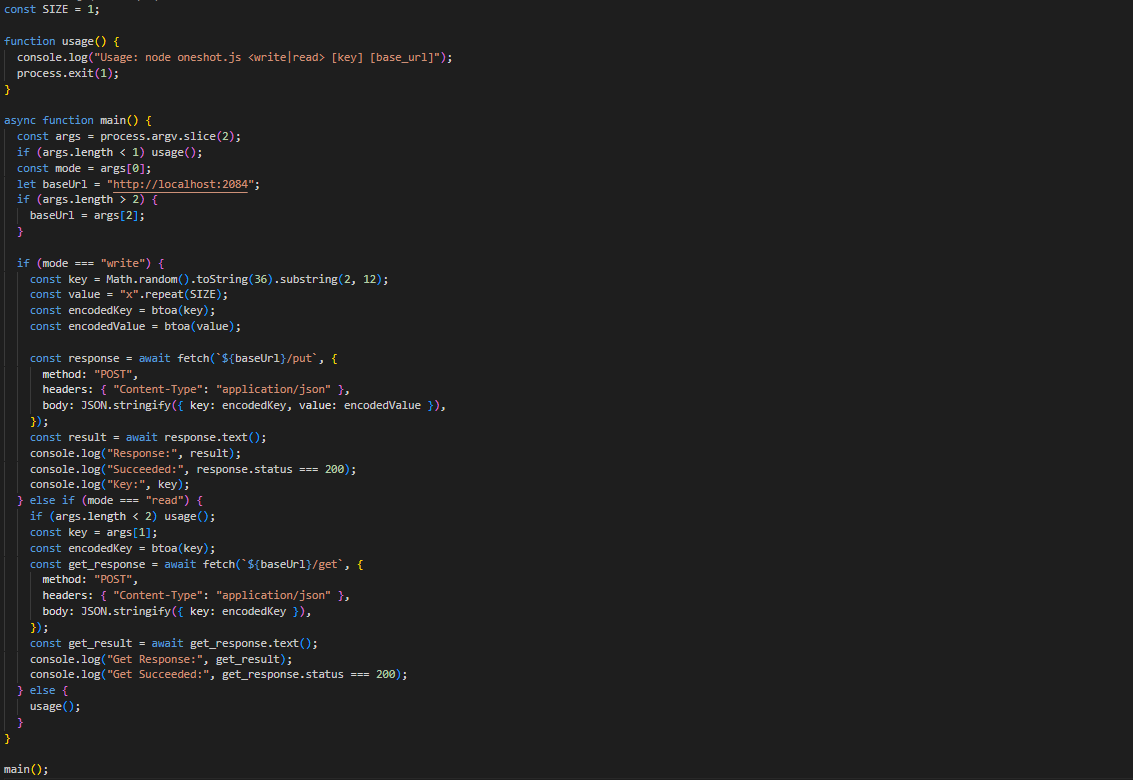
\includegraphics[width=0.95\textwidth]{resources/chapter-4/oneshot.png}
    \caption{Implementasi oneshot.js}
    \label{fig:implementasi-oneshot}
\end{figure}

Untuk verifikasi lebih lanjut, \textit{endpoint} /log dapat digunakan untuk melihat log yang dihasilkan oleh sistem. Khususnya untuk sistem \textit{erasure coding}, \textit{endpoint} ini akan memperlihatkan informasi mengenai data yang telah di-\textit{encode}.